\documentclass[12pt,a4paper]{article}
\usepackage{listings}
\usepackage{xcolor}

\definecolor{codegreen}{rgb}{0,0.6,0}
\definecolor{codegray}{rgb}{0.5,0.5,0.5}
\definecolor{codepurple}{rgb}{0.58,0,0.82}
\definecolor{backcolour}{rgb}{0.95,0.95,0.92}

\lstdefinestyle{mystyle}{
    % backgroundcolor=\color{backcolour},   
    commentstyle=\color{codegreen},
    keywordstyle=\color{magenta},
    % numberstyle=\tiny\color{codegray},
    stringstyle=\color{codepurple},
    basicstyle=\ttfamily\footnotesize,
    breakatwhitespace=false,         
    breaklines=true,                 
    captionpos=b,                    
    keepspaces=true,                 
    % numbers=left,                    
    % numbersep=5pt,                  
    showspaces=false,                
    showstringspaces=false,
    showtabs=false,                  
    tabsize=2
}

\lstset{style=mystyle}

\usepackage{enumerate}
\usepackage{graphicx}
\graphicspath{ {./images/} }
\usepackage{pgf}
\usepackage{svg}
\usepackage{tikz}
\usepackage{stanli}
\usepackage{afterpage}
\usepackage{multirow}
\usepackage{subfig}
\usepackage{pgfpages}
\usepackage{svg}
\usepackage{rotating}
\usepackage{graphicx,parskip,appendix,float}
\def\@submitdate{\number\the\day\space\space
  \ifcase\the\month\or
  January\or February\or March\or April\or May\or June\or
  July\or August\or September\or October\or November\or December\fi
  \space \number\the\year}

\pgfpagesdeclarelayout{boxed}
{
    \edef\pgfpageoptionborder{0pt}
}
% Border Settings
{
    \pgfpagesphysicalpageoptions
    {%
        logical pages=1,%
    }
    \pgfpageslogicalpageoptions{1}
    {
        border code=\pgfsetlinewidth{0.5pt}\pgfstroke,%
        border shrink=\pgfpageoptionborder,%
        resized width=.9\pgfphysicalwidth,%
        resized height=.9\pgfphysicalheight,%
        center=\pgfpoint{.5\pgfphysicalwidth}{.5\pgfphysicalheight}%
    }%
}

\pgfpagesuselayout{boxed}

\usepackage[english]{babel}

\usepackage[a4paper,top=1.5cm,bottom=1.5cm,left=1.5cm,right=1.5cm,marginparwidth=1cm]{geometry}

% Useful packages
\usepackage{amsmath}
\usepackage{graphicx}
\usepackage[colorlinks=true, allcolors=blue]{hyperref}

\title{}
\author{}
\date{}

\begin{document}
	
\newcommand{\subf}[2]{%
    {\small\begin{tabular}[t]{@{}c@{}}
            #1\\#1
    \end{tabular}}%
}

\begin{titlepage}
    \begin{center}
        \vspace{1cm}		
        \Huge
        \textbf{EN3160 - Image Processing and Machine Vision}

        \vspace{0.5cm}
        %\Huge
        {\LARGE Assignment 02 on Fitting and Alignment
Filtering}
        \vspace{1cm}
        \large			
        \vspace{0.5cm}
        \LARGE			
        \vspace{3cm}
        
        \textbf{}
        
\includegraphics[width=0.3\textwidth]{university.png}\\
        {\Large University of Moratuwa}
        \\
        {\Large Sri Lanka}
        \vfill			
        \vspace{0.4cm}
        \Large
    \end{center}
    
    \Large
    \vspace{1cm}
    \begin{tabbing}
        \hspace*{11em}\= \hspace*{4em} \= \kill % set the tabbings
        %\> Group \> : Group D \\
        \> Name\> :  Abithan A.\\
        \> Reg No\>:  210019E \\
    \end{tabbing}
    % \begin{figure}[!b]
    % \begin{center}
    % Copyright \copyright\; 2011 Dan Eiblum\\
    % All rights reserved\\
    
    % ISBN: 978-1-4610-9314-5\\
    % \textbf{Library of Congress Control Number: 2011905974}
    % \end{center}
    % \end{figure}
     \centering
    % \@submitdate \\
    \href{https://github.com/Abithan07/Fitting-and-Alignment}{\normalsize{https://github.com/Abithan07/Fitting-and-Alignment}}
    
    \vspace{8mm}
    
\includegraphics[height=10mm]{ent.png}
\end{titlepage}

%%%%%%%%%%%%%%%%%%%%%%%%%%%%%%%%%%%%%%%%%%%%%%%%%%%%%%%%%%%%%%%%%%%%%%%%%%%	

\section{Question 1}

    \begin{figure}[H]
        \centering
        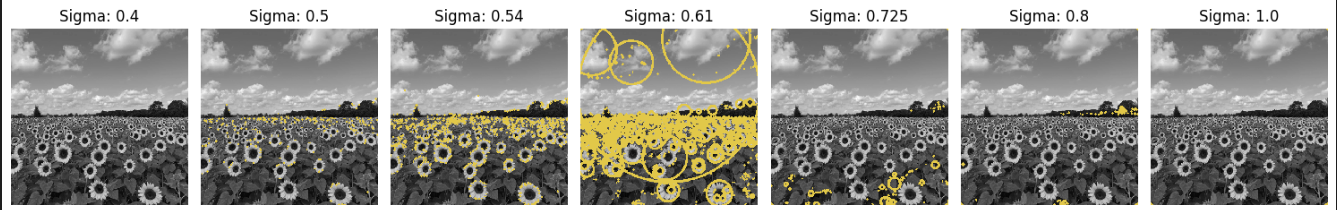
\includegraphics[width=0.9\linewidth]{images/Screenshots/1.png}
        \caption{Detected blobs for different sigma values}
        \label{fig:enter-label}
    \end{figure}

    \begin{itemize}
        \item Maximum radius got : 185
        \item Range of $\sigma$ values : [0.4, 0.5, 0.54, 0.61, 0.725, 0.8, 1.0]
        \item Selected $\sigma$ value : 0.61
    \end{itemize}
    

\section{Question 2}

\lstinputlisting[language=python]{Code/2_1.py}
    \begin{figure}[H]
        \centering
        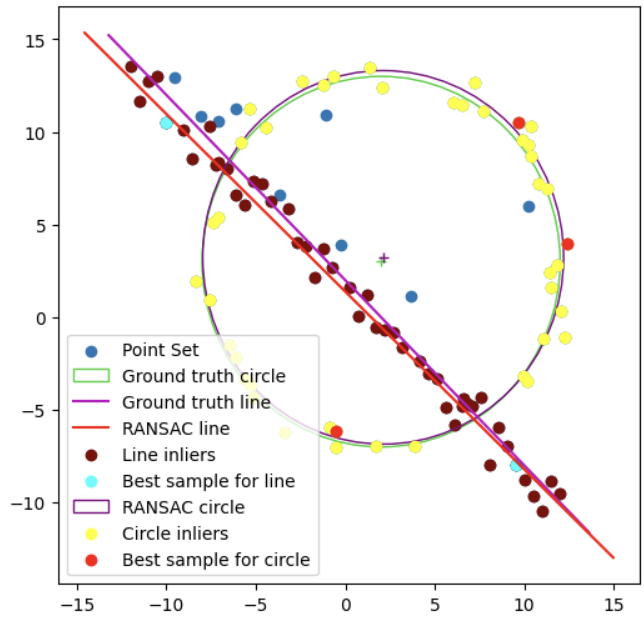
\includegraphics[width=0.5\linewidth]{images/Screenshots/2.png}
        \caption{Best fit and Grown truth line and circle.}
        \label{fig:enter-label}
    \end{figure}

This approach includes fitting a line to the noisy points using the RANSAC algorithm and subtracting it. This cleans up the circle fitting by picking relevant inliers. Otherwise, in case we apply RANSAC to fit the circle first, it may include random points from line inliers and hence fits inaccurately.



\section{Question 3}
    
    \lstinputlisting[language=python]{Code/3.py}
    
    \begin{figure}[H]
        \centering
        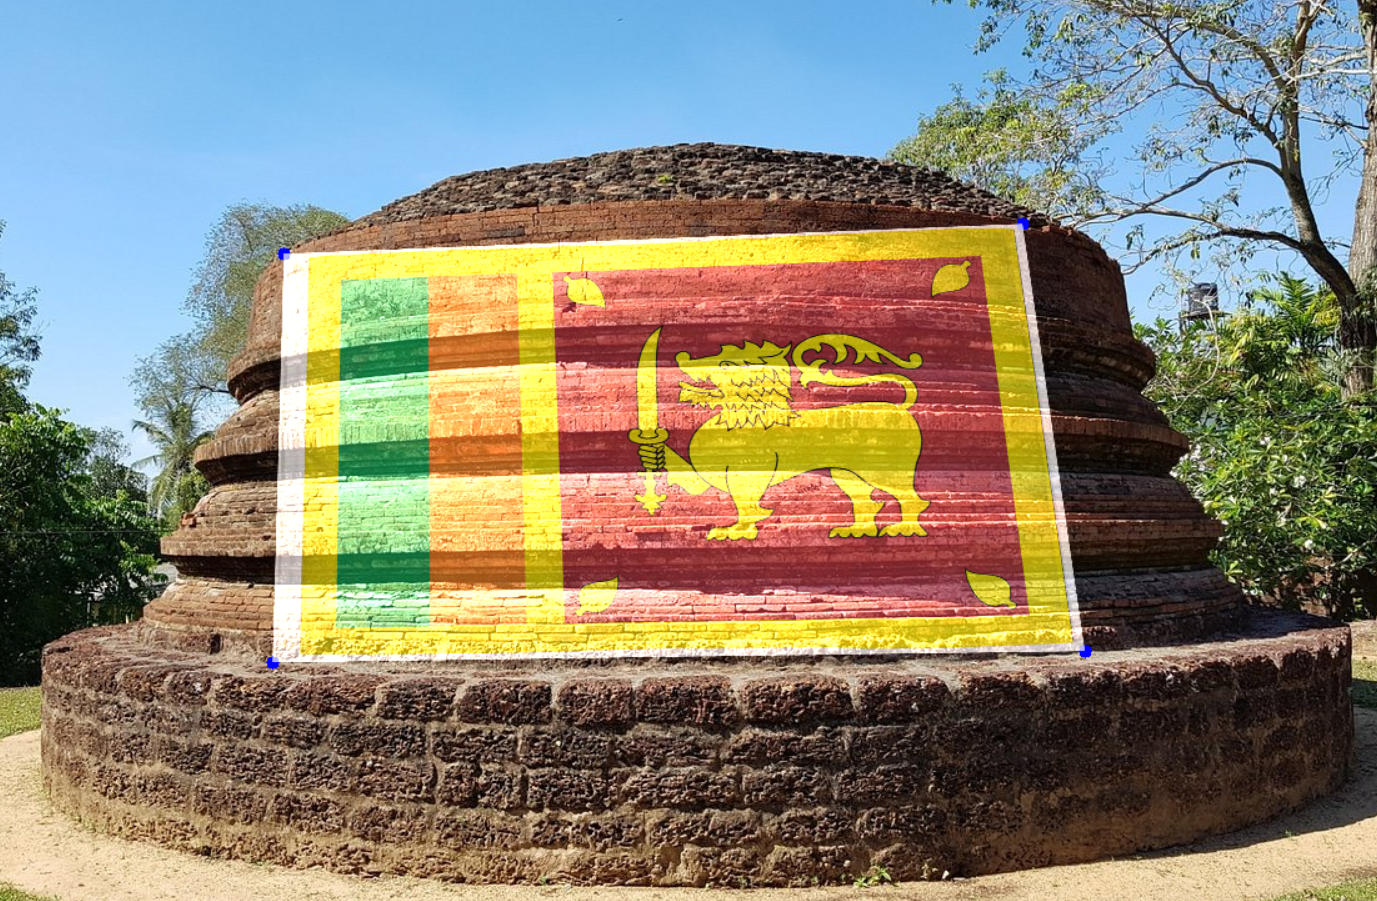
\includegraphics[width=0.5\linewidth]{images/Screenshots/3_1.png}
        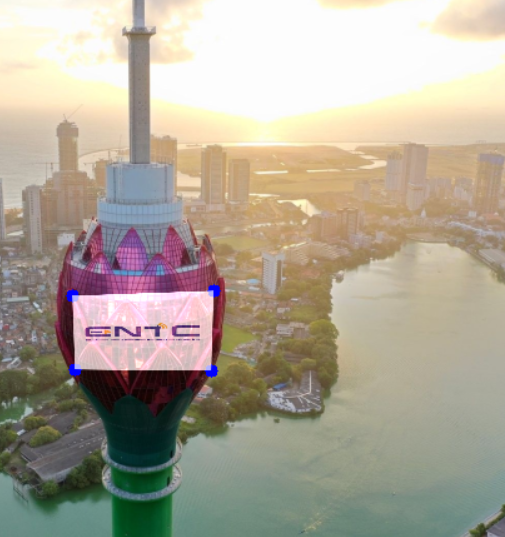
\includegraphics[width=0.4\linewidth]{images/Screenshots/3_2.png}
        \caption{Superposition Examples}
        \label{fig:enter-label}
    \end{figure}


    

\section{Question 4}

\subsection{a.}
    \begin{figure}[H]
        \centering
        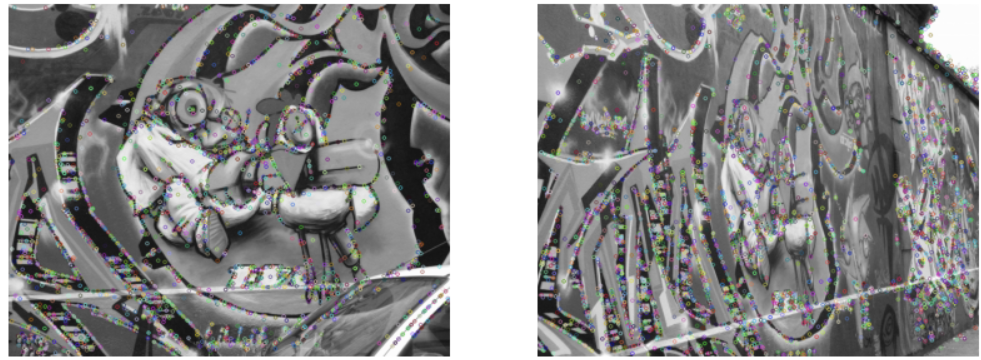
\includegraphics[width=0.85\linewidth]{images/Screenshots/4_11.png}
        \caption{Matched Keypoints}
        \label{fig:enter-label}
    \end{figure}

    \begin{figure}[H]
        \centering
        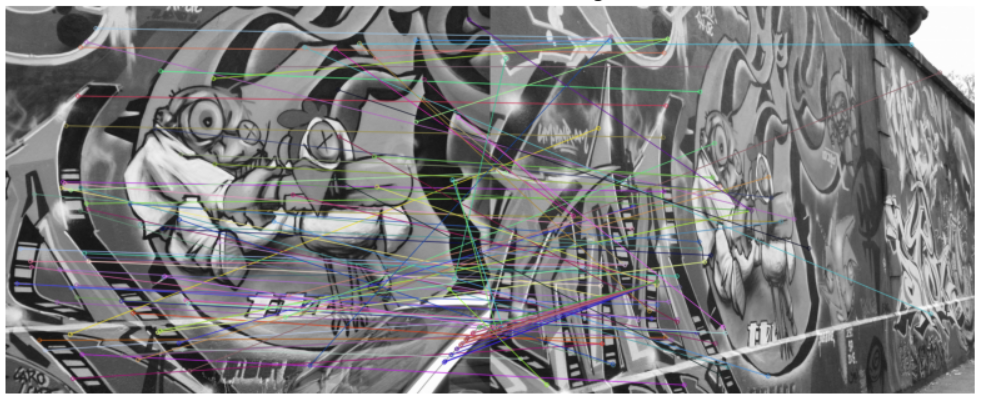
\includegraphics[width=0.85\linewidth]{images/Screenshots/4_12.png}
        \caption{Feature Matches}
        \label{fig:enter-label}
    \end{figure}

\subsection{b.}
     \begin{figure}[H]
        \centering
        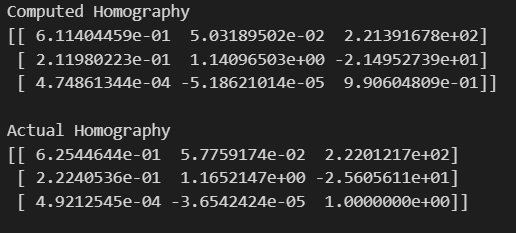
\includegraphics[width=0.85\linewidth]{images/Screenshots/4_2.png}
        \caption{Computed and Actual Homography}
        \label{fig:enter-label}
    \end{figure}
    
    %Sum of squared errors: 17.280918220859423

\subsection{c.}

    % \begin{figure}[H]
    %     \centering
    %     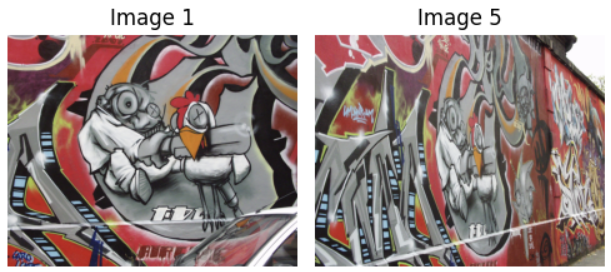
\includegraphics[width=0.85\linewidth]{images/Screenshots/4_31.png}
    %     \caption{Images}
    %     \label{fig:enter-label}
    % \end{figure}

    \begin{figure}[H]
        \centering
        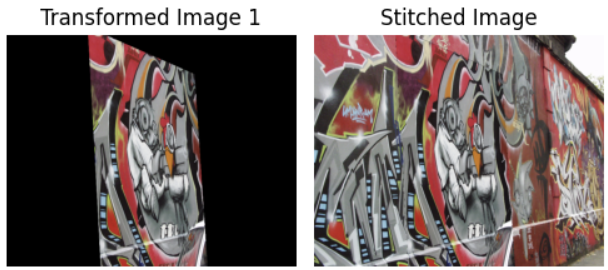
\includegraphics[width=0.85\linewidth]{images/Screenshots/4_32.png}
        \caption{Transformed and Stitched Images}
        \label{fig:enter-label}
    \end{figure}

\end{document}
